\documentclass[UTF8]{article}
\usepackage{graphicx}
\usepackage{subfigure}
\usepackage{amsmath}
\usepackage{makecell}
\usepackage[utf8]{inputenc}
\usepackage[space]{ctex} %中文包
\usepackage{listings} %放代码
\usepackage{xcolor} %代码着色宏包
\usepackage{CJK} %显示中文宏包
\usepackage{float}
\usepackage{diagbox}
\usepackage{bm}
\usepackage{ulem} 
\usepackage{amssymb}
\usepackage{soul}
\usepackage{color}
\usepackage{geometry}
\usepackage{fancybox} %花里胡哨的盒子
\usepackage{xhfill} %填充包, 可画分割线 https://www.latexstudio.net/archives/8245
\usepackage{multicol} %多栏包
\usepackage{enumerate} %可以方便地自定义枚举标题
\usepackage{multirow} %表格中多行单元格合并
\usepackage{wasysym} %可以使用wasysym里的一堆奇奇怪怪的符号
\usepackage{hyperref} % url
%%%%%%%%%%%%%%%伪代码%%%%%%%%%%%%%%%
\usepackage{amsmath}
\usepackage{algorithm}
\usepackage{algorithmicx}
\usepackage[noend]{algpseudocode}
%%%%%%%%%%%%%%%画图包%%%%%%%%%%%%%%%
\usepackage{tikz}
\usepackage{pgfplots} % http://pgfplots.sourceforge.net/gallery.html
\usetikzlibrary{pgfplots.patchplots} % 拟合支持
\usetikzlibrary{arrows,shapes,automata,petri,positioning,calc} % 状态图支持
\usetikzlibrary{arrows.meta} % 箭头
\usetikzlibrary{shadows} % 阴影支持
\usepackage{forest} % 画树
\usepackage{adjustbox} % 旋转

\geometry{left = 1.5cm, right = 1.5cm, top=1.5cm, bottom=2cm}

\definecolor{mygreen}{rgb}{0,0.6,0}
\definecolor{mygray}{rgb}{0.5,0.5,0.5}
\definecolor{mymauve}{rgb}{0.58,0,0.82}
\lstset{
	backgroundcolor=\color{white}, 
	%\tiny < \scriptsize < \footnotesize < \small < \normalsize < \large < \Large < \LARGE < \huge < \Huge
	basicstyle = \footnotesize,       
	breakatwhitespace = false,        
	breaklines = true,                 
	captionpos = b,                    
	commentstyle = \color{mygreen}\bfseries,
	extendedchars = false,
	frame = shadowbox, 
	framerule=0.5pt,
	keepspaces=true,
	keywordstyle=\color{blue}\bfseries, % keyword style
	language = C++,                     % the language of code
	otherkeywords={string}, 
	numbers=left, 
	numbersep=5pt,
	numberstyle=\tiny\color{mygray},
	rulecolor=\color{black},         
	showspaces=false,  
	showstringspaces=false, 
	showtabs=false,    
	stepnumber=1,         
	stringstyle=\color{mymauve},        % string literal style
	tabsize=4,          
	title=\lstname           
}

%\sum\nolimits_{j=1}^{M}   上下标位于求和符号的水平右端, 
%\sum\limits_{j=1}^{M}   上下标位于求和符号的上下处, 
%\sum_{j=1}^{M}  对上下标位置没有设定, 会随公式所处环境自动调整. 

%%%%%%%%%%%%%画图包%%%%%%%%%%%%%
\usepackage{tikz}
%%%%%%%%%%%%%好看的矩形%%%%%%%%%%%%%
\tikzset{
	rect1/.style = {
		shape = rectangle,% 指定样式
		minimum height=2cm,% 最小高度
		minimum width=4cm,% 最小宽度
		align = center,% 文字居中
		drop shadow,% 阴影
	}
}
%%%%%%%%%%%%%画图背景包%%%%%%%%%%%%%
\usetikzlibrary{backgrounds}

%%%%%%%%%%%%%在tikz中画一个顶点%%%%%%%%%%%%%
%%%%%%%%%%%%%#1:node名称%%%%%%%%%%%%%
%%%%%%%%%%%%%#2:位置%%%%%%%%%%%%%
%%%%%%%%%%%%%#3:标签%%%%%%%%%%%%%
\newcommand{\newVertex}[3]{\node[circle, draw=black, line width=1pt, scale=0.8] (#1) at #2{#3}}
%%%%%%%%%%%%%在tikz中画一条边%%%%%%%%%%%%%
\newcommand{\newEdge}[2]{\draw [black,very thick](#1)--(#2)}
%%%%%%%%%%%%%在tikz中放一个标签%%%%%%%%%%%%%
%%%%%%%%%%%%%#1:名称%%%%%%%%%%%%%
%%%%%%%%%%%%%#2:位置%%%%%%%%%%%%%
%%%%%%%%%%%%%#3:标签内容%%%%%%%%%%%%%
\newcommand{\newLabel}[3]{\node[line width=1pt] (#1) at #2{#3}}

%%%%%%%%%%%%%强制跳过一行%%%%%%%%%%%%%
\newcommand{\jumpLine} {\hspace*{\fill} \\}
%%%%%%%%%%%%%关键点指令,可用itemise替代%%%%%%%%%%%%%
\newcommand{\keypoint}[2]{$\bullet$\textbf{#1}\quad#2\par}
%%%%%%%%%%%%%<T>平均值表示%%%%%%%%%%%%%
\newcommand{\average}[1]{\left\langle #1\right\rangle }
%%%%%%%%%%%%%表格内嵌套表格%%%%%%%%%%%%%
\newcommand{\tabincell}[2]{\begin{tabular}{@{}#1@{}}#2\end{tabular}}
%%%%%%%%%%%%%大黑点item头%%%%%%%%%%%%%
\newcommand{\itemblt}{\item[$\bullet$]}
%%%%%%%%%%%%%大圈item头%%%%%%%%%%%%%
\newcommand{\itemc}{\item[$\circ$]}
%%%%%%%%%%%%%大星星item头%%%%%%%%%%%%%
\newcommand{\itembs}{\item[$\bigstar$]}
%%%%%%%%%%%%%右▷item头%%%%%%%%%%%%%
\newcommand{\itemrhd}{\item[$\rhd$]}
%%%%%%%%%%%%%定义为%%%%%%%%%%%%%
\newcommand{\defas}{=_{df}}
%%%%%%%%%%%%%偏导%%%%%%%%%%%%%
\newcommand{\partialx}[2]{\frac{\partial #1}{\partial #2}}
%%%%%%%%%%%%%蕴含%%%%%%%%%%%%%
\newcommand{\imp}{\rightarrow}
%%%%%%%%%%%%%上取整%%%%%%%%%%%%%
\newcommand{\ceil}[1]{\lceil#1\rceil}
%%%%%%%%%%%%%下取整%%%%%%%%%%%%%
\newcommand{\floor}[1]{\lfloor#1\rfloor}

%%%%%%%%%%%%%双线分割线%%%%%%%%%%%%%
\newcommand*{\doublerule}{\hrule width \hsize height 1pt \kern 0.5mm \hrule width \hsize height 2pt}
%%%%%%%%%%%%%双线中间可加东西的分割线%%%%%%%%%%%%%
\newcommand\doublerulefill{\leavevmode\leaders\vbox{\hrule width .1pt\kern1pt\hrule}\hfill\kern0pt }
%%%%%%%%%%%%%左大括号%%%%%%%%%%%%%
\newcommand{\leftbig}[1]{\left\{\begin{array}{l}#1\end{array}\right.}
%%%%%%%%%%%%%矩阵%%%%%%%%%%%%%
\newcommand{\mat}[2]{\left[\begin{array}{#1}#2\end{array}\right]}
%%%%%%%%%%%%%可换行圆角文本框%%%%%%%%%%%%%
\newcommand{\ovalboxn}[1]{\ovalbox{\tabincell{l}{#1}}}
%%%%%%%%%%%%%设置section的counter, 使从1开始%%%%%%%%%%%%%
\setcounter{section}{0}

%%%%%%%%%%%%%Colors%%%%%%%%%%%%%
\newcommand{\lightercolor}[3]{% Reference Color, Percentage, New Color Name
	\colorlet{#3}{#1!#2!white}
}
\newcommand{\darkercolor}[3]{% Reference Color, Percentage, New Color Name
	\colorlet{#3}{#1!#2!black}
}
\definecolor{aquamarine}{rgb}{0.5, 1.0, 0.83}
\definecolor{Seashell}{RGB}{255, 245, 238} %背景色浅一点的
\definecolor{Firebrick4}{RGB}{255, 0, 0}%文字颜色红一点的
\lightercolor{gray}{20}{lgray}
\newcommand{\hlg}[1]{
	\begingroup
	\sethlcolor{lgray}%背景色
	\textcolor{black}{\hl{\mbox{#1}}}%textcolor里面对应文字颜色
	\endgroup
}
\lightercolor{red}{20}{lred}
\lightercolor{black}{20}{lblack}
\lightercolor{black}{60}{mblack}

\title{并行计算 HW3 及 HW4}
\author{PB18111697 王章瀚}

\begin{document}
\maketitle
\section*{1.}
\noindent \textbf{在 PRAM-CREW 模型上, 用 n 个处理器在 O(1) 时间内求出数组 $A[1..n]=\{0,\cdots,0,1,\cdots,1\}$ 中最先为 1 值的下标, 写出并行伪代码.} \\ \jumpLine

\begin{algorithm}[H]
	\caption{{\sc First-One-Index}($A$)}
	\begin{algorithmic}[1] %每行显示行号
		\Require 数组 $A[1..n]=\{0,\cdots,0,1,\cdots,1\}$
		\Function {\sc First-One-Index}{$A$}
			\For{$i=1..n-1$ \textbf{par-}}
				\If {$A[i]$ == 0 and $A[i+1]$ == 1}
					\State \Return i + 1
				\EndIf
			\EndFor
		\EndFunction
	\end{algorithmic}
\end{algorithm}

\section*{7.3.}
\subsection*{(1).}
\noindent \textbf{试分析算法 7.3 的时间复杂度.} \\ \jumpLine\noindent
先按步说明:
\begin{enumerate}[(1).]
	\item 显然 O(1)
	\item 循环并行化后, 每个循环体内需要求 rank, 这最多需要 $\Theta(n)$, 但是如果能够给出 $n$ 个进程, 就能在 O(1) 内判断出 $b_{i\log m}$ 在 $A$ 中的 rank.
	\item 每个并行体内均是数据拷贝, 共需要 $\Theta(\log m + j(i + 1) - j(i))$, 这其实是 $O(\log m + n)$ 的.(这是因为如果 $a_1$ 大于 $B$ 中所有元素, 则有一个进程要拷贝 $n$ 个数据, 就算并行, 也需要等它完成它的任务, 这需要 $\Theta(n)$). 但如果 A 数据是均匀分布的, 就只需要 $\Theta(\log m + \frac{n}{m}\log m)$ 的时间.
\end{enumerate}
因此总共需要 $O(\log m + n)$. 若 A 元素比较均匀, 则是 $\Theta(\log m + \frac{n}{m}\log m)$.

\subsection*{(2).}
\noindent \textbf{
令 $A=\{0,1,2,7,9,11,16,17,18,19,23,24,25,27,28,30,33,34\}, B=\{3,4,5,6,8,10,12,13,14,15,20,21,22,26,29,31\}$. 试按算法 6.3 将其对数划分, 并最终将它们归并.} \\ \jumpLine\noindent
对此情况, $n=18$, $m=16$, $k(m)=m/\log m=4$,
\begin{enumerate}[(1).]
	\item $j(0)=0;\ j(k(m))=j(4)=18$
	\item 并行得到 
		\begin{itemize}
			\item $b_{1\log m}=b_{4}=6, j(1)=rank(b_4: A)=3$
			\item $b_{2\log m}=b_{8}=13, j(2)=rank(b_8: A)=6$
			\item $b_{3\log m}=b_{12}=21, j(3)=rank(b_{12}: A)=10$
%			\item $b_{4\log m}=b_{16}=31, j(4)=rank(b_{16}: A)=16$
		\end{itemize}
	\item 并行得到分组结果:
		\begin{itemize}
			\item $A_0=(0,1,2), B_0=(3,4,5,6)$
			\item $A_1=(7,9,11), B_1=(8,10,12,13)$
			\item $A_2=(16,17,18,19), B_2=(14,15,20,21)$
			\item $A_3=(23,24,25,27,28,30,33,34), B_3=(22,26,29,31)$
		\end{itemize}
\end{enumerate}
分段归并即得:
\begin{itemize}
	\item $(0,1,2,3,4,5,6)$
	\item $(7,8,9,10,11,12,13)$
	\item $(14,15,16,17,18,19,20,21)$
	\item $(22,23,24,25,26,27,28,29,30,31,33,34)$
\end{itemize}
拼接起来即:
$$(0,1,2,3,4,5,6,7,8,9,10,11,12,13,14,15,16,17,18,19,20,21,22,23,24,25,26,27,28,29,30,31,33,34)$$

\section*{7.6.}
\subsection*{(1).}
\noindent \textbf{试分析算法 7.9 的总运算量 W(n)} \\ \jumpLine\noindent
逐步说明:
\begin{enumerate}[(1). ]
	\item 初始化 $n$ 个进程计算量均为 $\Theta(1)$, 故总共是 $\Theta(n)$
	\item 对 $h$ 从 $1$ 到 $\log n$ 共 $\log n$ 次循环. 其内并行 $n/2^h$ 个进程, 每个经过 $\Theta(1)$ 的计算, 因此总共 $$\Theta(\sum\limits_{h=1}^{\log n} n/2^h)=\Theta(n(1-(\frac{1}{2})^{\log n}))=\Theta(n(1-\frac{1}{n})=\Theta(n)$$
	\item 类似地, $h$ 共 $\Theta(\log n)$ 层循环, 其内 $n/2^k$ 个进程内部各需要 $\Theta(1)$ 的操作, 总共是 $$\Theta(\sum\limits_{h=0}^{\log n} n/2^h)=\Theta(2n(1-(\frac{1}{2})^{\log n}))=\Theta(2n)$$
\end{enumerate}

因此总运算量是 $W(n)=\Theta(n+n + 2n)=\Theta(4n)$

\subsection*{(2).}
\noindent \textbf{假定序列为 (1,2,3,4,5,6,7,8), 试用算法 7.9 求其前缀和} \\ \jumpLine\noindent
按步说明:
\begin{enumerate}[(1). ]
	\item 初始化步, $B(0,1)=1, B(0,2)=2, \cdots, B(0,8)=8$, 即 B 如下表:
	\begin{center}
	\begin{tabular}{|c|c|c|c|c|c|c|c|}
		\hline
		1 & 2 & 3 & 4 & 5 & 6 & 7 & 8 \\
		\hline
		&  &  &  &  &  &  &  \\
		\hline
		&  &  &  &  &  &  &  \\
		\hline
		&  &  &  &  &  &  &  \\
		\hline
	\end{tabular}
	\end{center}
	\item 正向遍历时, 总将 $B(h,j)=B(h-1,2j-1) * B(h-1, 2j)$
	\begin{center}
		\begin{tabular}{|c|c|c|c|c|c|c|c|}
			\hline
			1 & 2 & 3 & 4 & 5 & 6 & 7 & 8 \\
			\hline
			3 &  & 7 &  & 11 &  & 15 &  \\
			\hline
			10 &  &  &  & 26 &  &  &  \\
			\hline
			36 &  &  &  &  &  &  &  \\
			\hline
		\end{tabular}
	\end{center}
	\item 反向遍历时, 即能根据 $B$ 求出 $C$:
	\begin{center}
		\begin{tabular}{|c|c|c|c|c|c|c|c|}
			\hline
			1 & 3 & 6 & 10 & 15 & 21 & 28 & 36 \\
			\hline
			3 &  & 10 &  & 21 &  & 36 &  \\
			\hline
			10 &  &  &  & 36 &  &  &  \\
			\hline
			36 &  &  &  &  &  &  &  \\
			\hline
		\end{tabular}
	\end{center}
\end{enumerate}
$C$ 的第一行即为前缀和

\section*{2.6}
\begin{center}
	\begin{figure}[H]
		\centering
		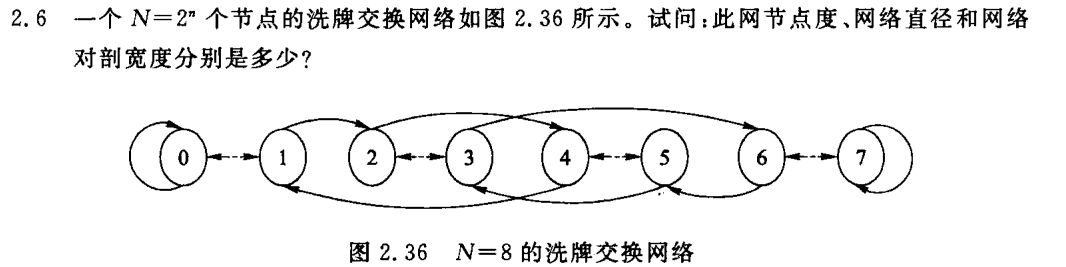
\includegraphics[width=\linewidth]{image/2.6.png}
	\end{figure}
\end{center}

\begin{itemize}
	\item 节点度: 入射边和出射边之和. 每个节点在交换网络有两个度, 在洗牌网络有两个度, 总共节点度是 4.
	\item 网络直径: 网络中任何两个节点之间的最长距离. 如 N=8, 则应为节点路径 $0\rightarrow 1\rightarrow 2\rightarrow 3 \rightarrow 6 \rightarrow 7$ 是最长的之一, 其长度为 5. 对于 $N=2^n$ 也类似, 最远的应该是节点 0 到节点 N-1, 路径应为交换, 洗牌不断轮流(即刚开始加 1, 然后每次乘 2 加 1), 因此其长度为 $2n-1$.
	\item 网络对剖宽度: 对分网络各半所需最少边数. 如分为 $\{0,1,2,3\}$ 和 $\{4,5,6,7\}$, 中间要划分开需要去掉最中间的 4 条边($2\rightarrow4, 3\rightarrow6,4\rightarrow1,5\rightarrow3$). 而对于 $N=2^n$ 的情况, 只要考虑 $0$ 到 $2^{n-1}-1$ 和 $2^{n-1}$ 到 $2^{n}-1$ 有多少条边即可. 因此对剖宽度为 $2^{n-1}$.
\end{itemize}

\section*{2.7}
\begin{center}
\begin{figure}[H]
	\centering
	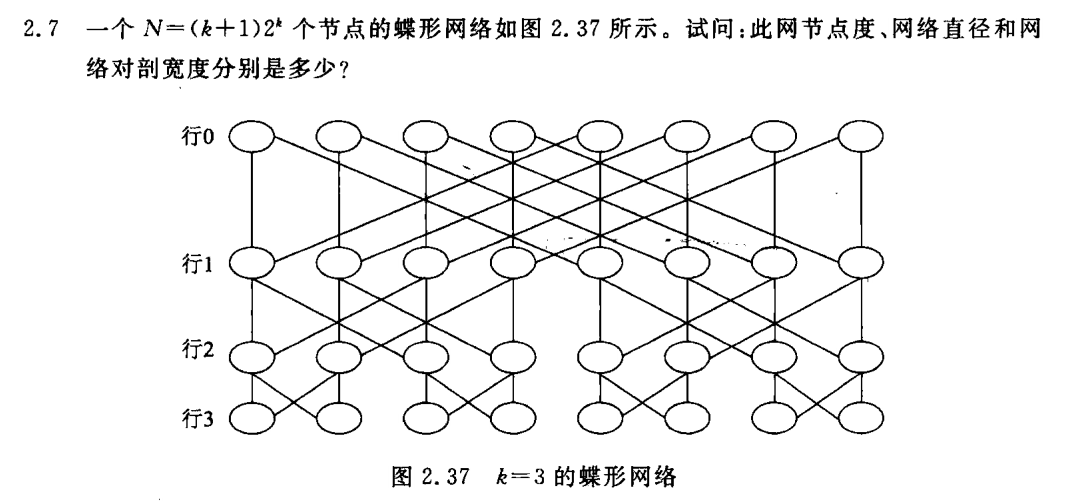
\includegraphics[width=\linewidth]{image/2.7.png}
\end{figure}
\end{center}

\begin{itemize}
\item 节点度: 入射边和出射边之和. 本网络是无向图. 第0行和最后一行每个节点都是 2 个边, 其节点度是 2; 而中间的行节点度都是 4.
\item 网络直径: 网络中任何两个节点之间的最长距离. 从行0第一个节点到最后一个节点需要先传播到行k再回到行0, 是最长路径的之一, 长度为 $2k$. (图中情况 $2k=6$)
\item 网络对剖宽度: 对分网络各半所需最少边数. 从中间对剖下去, 需要去掉 $2\times 2^{k-1}=2^k$ 条边, 因此对剖宽度是 $2^k$. (图中情况 $2^k=8$)
\end{itemize}

\section*{2.15}
\begin{center}
\begin{figure}[H]
	\centering
	
\includegraphics[width=\linewidth]{image/2.15.png}
\end{figure}
\end{center}
\begin{center}
\begin{figure}[H]
	\centering
	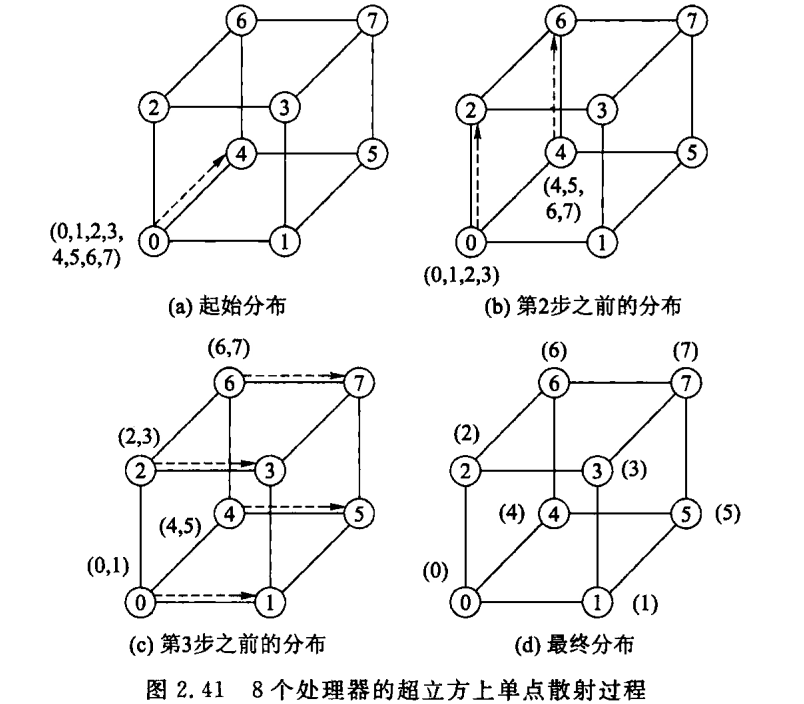
\includegraphics[width=\linewidth*2/3]{image/2.15.image.png}
\end{figure}
\end{center}

依据公式有:
$$t_{comm}(SF)=t_s+(mt_w+t_h)l$$
$$t_{comm}(CT)=t_s+mt_w+lt_h$$
其中 $t_s$ 是启动时间, $t_h$ 是节点延迟时间, $t_w$ 是字传输时间, 信包大小为 $m$, 链路数为 $l$.

具体到此题中, 可以忽略 $t_h$. 而由于本题中的传播过程每步都是传播一跳, 因此使用 CT 并不会有优势, 每次都仍然需要建立链路. 

另外, 每步传输都将可以 drop 一半的包, 每次传播也都涉及了 2 倍的节点. 因此第 $i$ 步, 需要传播包大小为 $\frac{p}{2^i}$, 总共传播 $\log p$ 次(即 $i=1, 2, \cdots, \log p - 1$, 因为是超立方, $p$ 为 2 的幂). 因此第 $i$ 次传播用的时间为 $t_s + mt_w\frac{p}{2^i}$

由此可知, 总时间为 
\begin{align*}
	t_{one-to-all-pers}&=t_s\log p + \sum\limits_{i=1}^{\log p} mt_w\frac{p}{2^i} \\
	&=t_s\log p + \sum\limits_{i=1}^{\log p} mt_w{2^i}\\
	&=t_s\log p + mt_w2^{\log p}-1 \\
	&=t_s\log p+mt_w(p-1)
\end{align*}





\end{document}









